\documentclass[border=10pt]{standalone}
\usepackage{pgfplots}
\pgfplotsset{compat=1.18}
\begin{document}
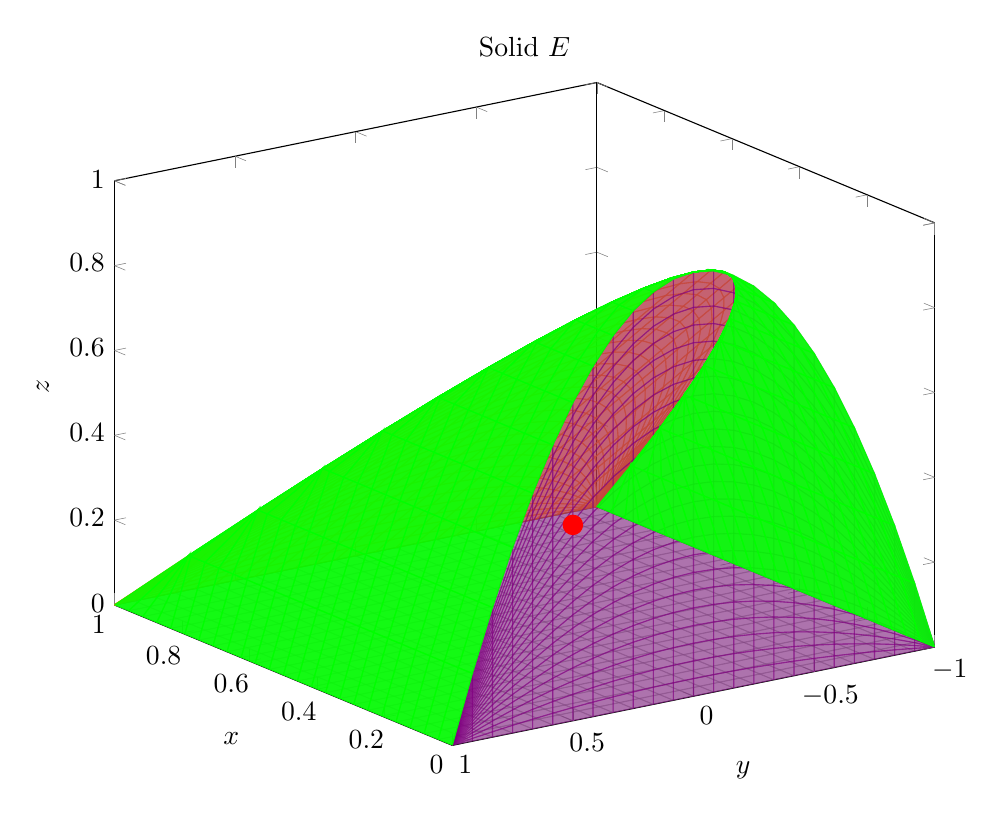
\begin{tikzpicture}
\begin{axis}[
    width=12cm, height=10cm,
    xlabel={$x$}, ylabel={$y$}, zlabel={$z$},
    view={-125}{22},
    xmin=0, xmax=1, ymin=-1, ymax=1, zmin=0, zmax=1,
    title={Solid $E$}]
% bottom face: z = 0 rectangle
\addplot3[surf, shader=flat, gray, opacity=0.35, domain=0:1, y domain=-1:1] (x, y, 0);
% back face: x + z = 1, parametrized by y in [-1,1], s in [0,1]: z = s(1-y^2), x = 1-z
\addplot3[surf, shader=flat, orange, opacity=0.6, domain=-1:1, y domain=0:1]
    ({1 - y*(1-x^2)}, {x}, {y*(1-x^2)});
% front face: x = 0, parametrized by y in [-1,1], s in [0,1]: z = s(1-y^2)
\addplot3[surf, shader=flat, violet, opacity=0.45, domain=-1:1, y domain=0:1]
    (0, {x}, {y*(1-x^2)});
% top curved face: z = 1-y^2 with 0 <= x <= y^2
\addplot3[surf, shader=flat, green, opacity=0.9, domain=0:1, y domain=-1:1]
    ({min(x, y^2)}, y, {1-y^2});
% center of mass
\addplot3[only marks, mark=*, red, mark size=3.5pt] coordinates {(0.3571, 0, 0.2857)};
\end{axis}
\end{tikzpicture}
\end{document}